\documentclass[a4paper,10pt]{article}
\usepackage[utf8]{inputenc}
\usepackage{amsmath, amsfonts, graphicx}
\usepackage{hyperref, indentfirst}
\usepackage{bbold}
%opening
\title{$\mathbb{RP^2}$ and photography}
\author{}
\newcommand{\diag}{\mathop{\mathrm{diag}}}
%\vspace{-15ex}
\date{}


\begin{document}
\maketitle
\section{Introducrion}




\section{$\mathbb{RP}^2$}


The directions of the axes $\xi_1$ and $x_1$ coincide in the world $\mathbb{R}^3$ as well as those for the axes  $\xi_2$ and $x_2$. The axis $x_3$ is pointed from the viewer and coincides with the principal axis of the camera lens. 

The form of the projection \eqref{cameraprojection} hints that we can think about a photo as about a chart of $\mathbb{RP}^2$. Indeed, all points on a line passing through the center of the lens (the coordinate origin) are projected on a single point on the camera sensor. A line in the world $\mathbb{R}^3$ on the photo is indistinguishable from a plane passing through the lens center and containing that line.  

In the section below I will prove the following statement. Let us have $n$ pairs of parallel lines on a plane in the $\mathbb{R}^3$; we can draw them on the paper and put on a table. If we make a photo of those lines from an arbitrary perspective they will intersect. The interesting fact about  the intersection points is that they all lie on a single line!

\section{$\mathbb{RP}^2$ }
 Real projective space $\mathbb{RP}^2$ is the space of lines in $\mathbb{R}^{3}$ passing through the origin. The coordinates of $\mathbb{R}^3$ $(x,y,z)$ are homogeneous coordinates of $\mathbb{RP}^2$, i.e. a point $(x,y,z)$ and all points $s(x,y,z)$, $s\neq 0$ correspond to a point of $\mathbb{RP}^2$.  

Planes in $\mathbb{R}^3$ passing through the origin are defined as 
\begin{equation}
\sum a_i x_i \equiv a\cdot x= 0.
\end{equation}
 Obviously, the quantities $a_i$ are defined up to an arbitrary multiplier and hence, the planes form a dual $\mathbb{RP}^2$. 
 
 Consider a chart of $\mathbb{RP}^2$
 \begin{equation}
 \xi_1 = \frac{x_1}{x_3}, \quad \xi_2=\frac{x_2}{x_3}, \quad x_3\neq 0\label{chart}
 \end{equation}
 
A plane $a$ is projected on this chart as a line

\begin{equation}
a_1 \xi_1 + a_2 \xi_2 + a_3 = 0
\end{equation} 

Here and further we will refer to planes $a$ as "lines" meaning their projection on the certain chart. However, we should always keep in mind that not all planes have their projection on the chart. In particular, the plain 
\begin{equation}
n^{(\infty)} = (0,0,1), \quad \text{or} \quad x_3 = 0\label{z0}
\end{equation}
does not project on the chart \eqref{chart} and therefore cannot be referred as a "line". In the science of Computer Vision they call it a "line at infinity" (hence the superscript).

Two lines on $\mathbb{RP}^2$ $a$ and $b$ are parallel on the chart  \eqref{chart} if 
\begin{equation}
(a\times b )\cdot n^{(\infty)} = 0, \quad \label{parallel}
\end{equation}
Alternatively, the lines on $\mathbb{RP}^2$ intersect in the point 
\begin{equation}
x = a \times b\label{intersectionpoint}
\end{equation}

In the language of lines and planes in $\mathbb{R}^3$ this can be interpreted as follows. Obviously, any two planes passing through the origin intersect. The intersection of the planes is the line \eqref{intersectionpoint} passing through the origin. If the intersection line lies in the plane \eqref{z0} then the projections of the planes on the chart \eqref{chart} are parallel.

The same result in the language of lines on the charts of $\mathbb{RP}^2$ is interpreted as  follows. The invariant form of \eqref{intersectionpoint} shows that, generally speaking, all lines on $\mathbb{RP}^2$ intersect, however if the condition \eqref{parallel} holds, then the intersection point is not  present on the considered chart.

Now let us consider the most generic invertable transformations 
\begin{equation}
x' = H x, \quad \det H \neq 0. 
\end{equation}

Obviously a plane $a$ under this transformation  is "moving in the opposite direction"
\begin{equation}
a'=H^{-T}a\label{cotransform}
\end{equation}

These kind of transformations are called homographies and clearly form a group. 

Now, let two lines $a$ and $b$ be parallel, i.e. satisfy \eqref{parallel},  and let $H$ be a homography such that

\begin{equation}
H^{-T} \cdot a,b,n^{(\infty)}  \neq \alpha n^{(\infty)} , \quad \forall \alpha \in \mathbb{R}
\end{equation}

 It is clear that the condition $\eqref{parallel}$ is not invariant under the transformation \eqref{cotransform}. Namely,

\begin{equation}
(a'\times b')\cdot  n^{(\infty)} \neq 0
\end{equation} 
 and, hence, the transformed lines $a'$ and $b'$ intersect in the point (see\eqref{intersectionpoint}):

\begin{equation}
x' = a' \times b'
\end{equation}

It is easy to show that 
\begin{equation}
(H^{-T}n^{(\infty)}) \cdot x'  = 0
\end{equation}
and, therefore, the point of $\mathbb{RP}^2$ $x'$ on the chart \eqref{chart} lies on the line $H^{-T}n^{(\infty)}$. 

Note, that while the plane $n^{(\infty)}$ does not have a projection on the chart \eqref{chart} the projection of the  transformed line $H^{-T}n^{(\infty)}$ is well defined. In other words, a generic homography moves the line at infinity.


\section{Result}

The result is illustrated in the Fig \ref{fig:drawed}

\begin{figure}[h]
\centering
 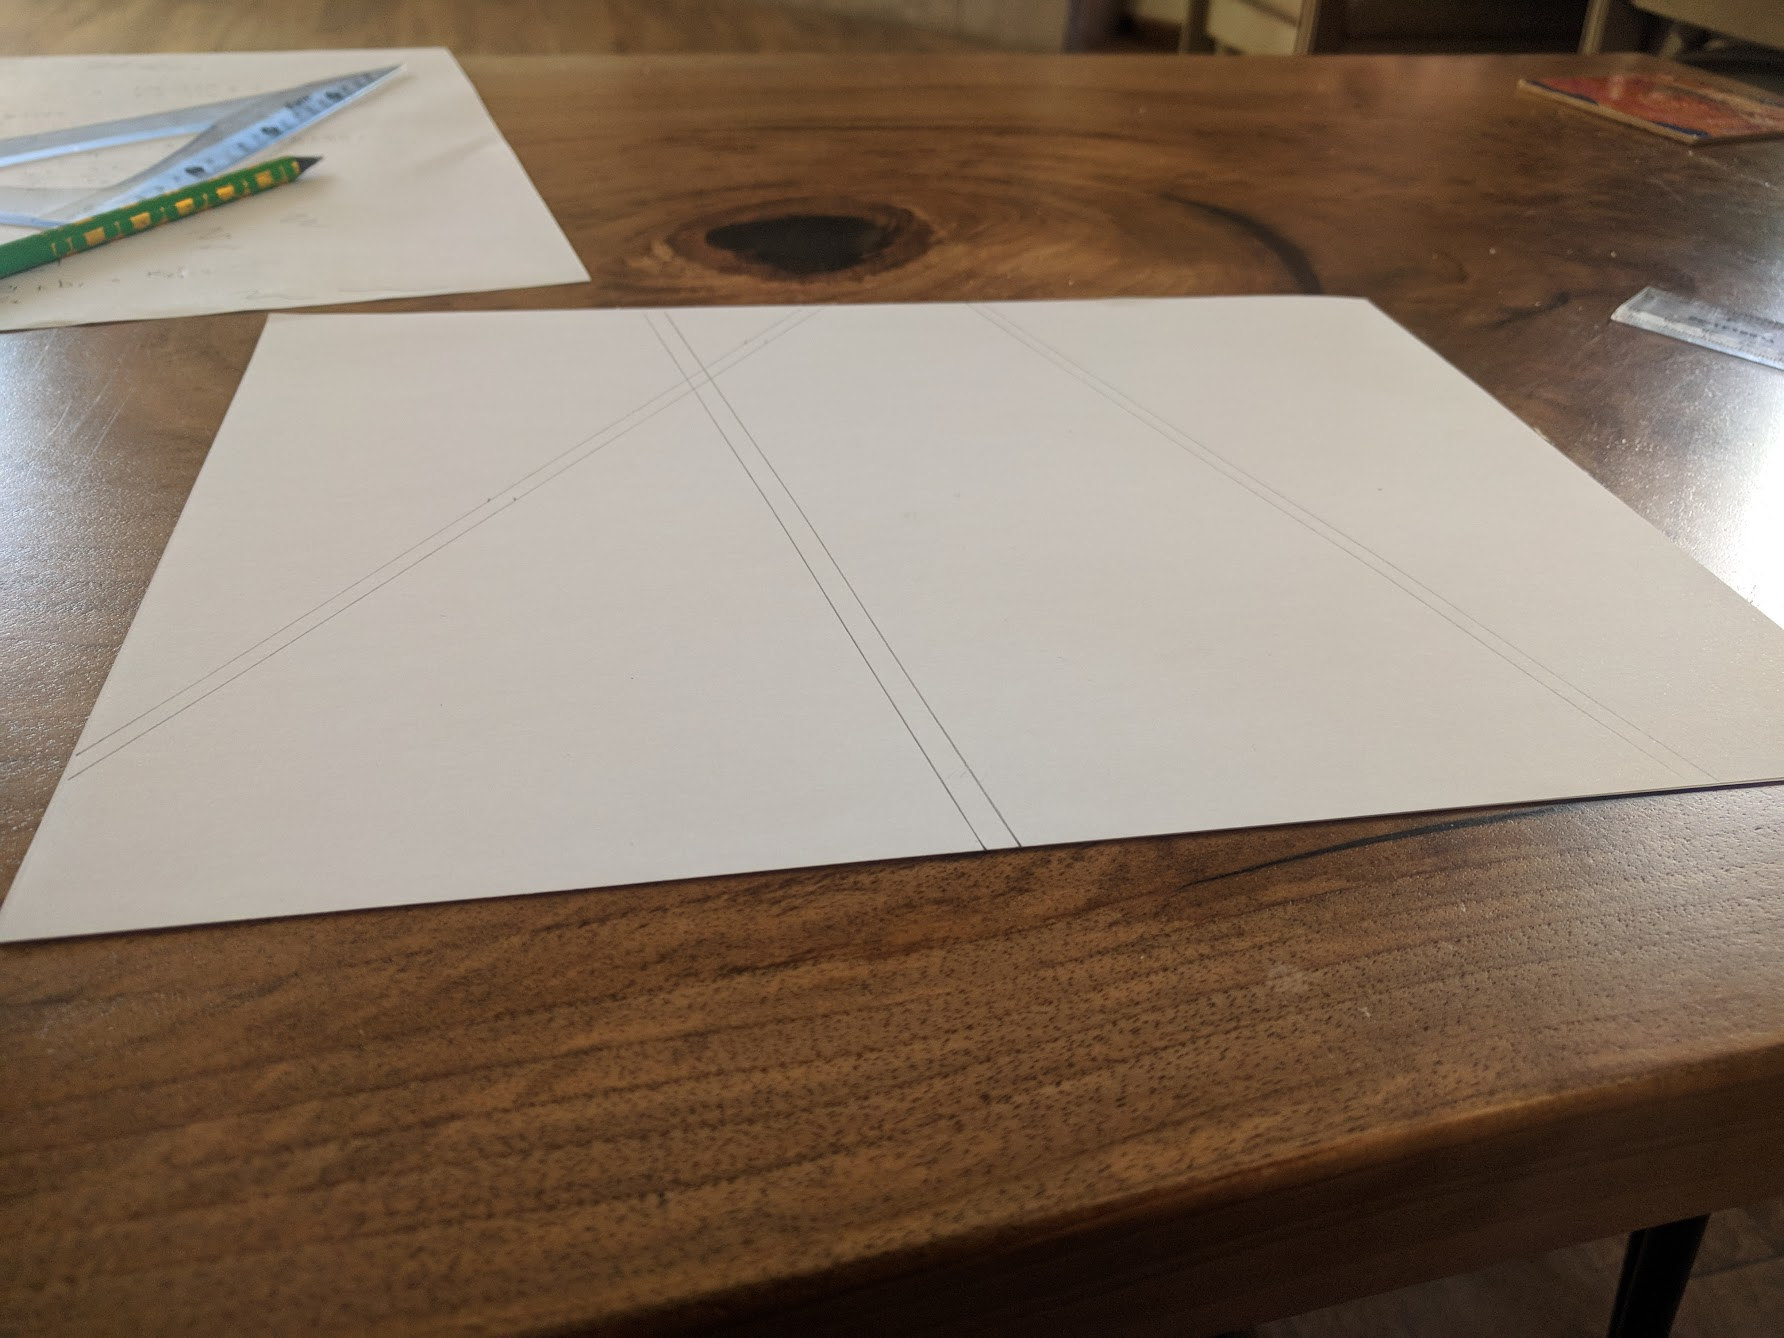
\includegraphics[width=0.6\textwidth]{../../images/parallel.jpg}
 \caption{Parallel lines taken from an arbitrary perspective. }
 \label{fig:3dcart}
\end{figure}

\begin{figure}[h]
\centering
 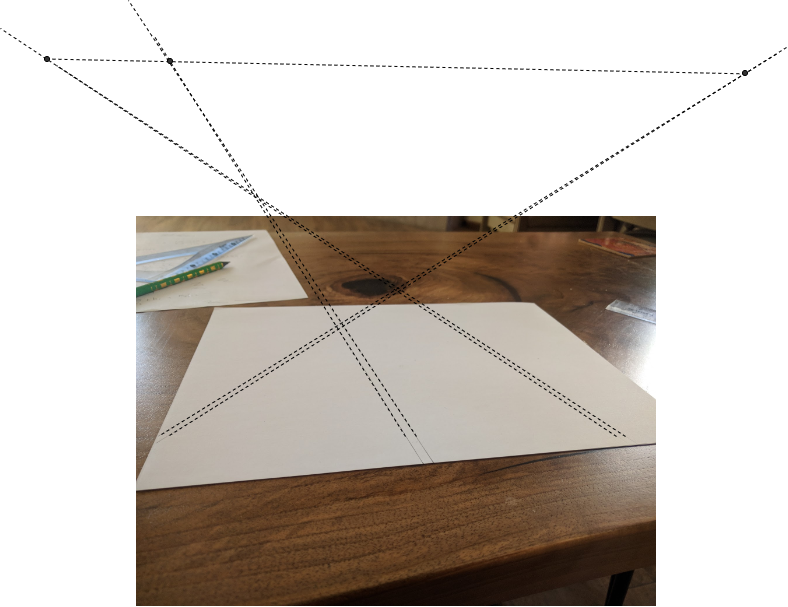
\includegraphics[width=0.9\textwidth]{../../images/parallel.png}
 \caption{The parallel lines intersect on the line at infinity. }
 \label{fig:drawed}
\end{figure}

\begin{thebibliography}{1}
\bibitem{mhopkins} Hopkins M.J. (1989) Minimal atlases of real projective spaces. In: Carlsson G., Cohen R., Miller H., Ravenel D. (eds) Algebraic Topology. Lecture Notes in Mathematics, vol 1370. Springer, Berlin, Heidelberg
\end{thebibliography}


\end{document}


